\section{System Overview}
\label{text:approach/overview}
As shown in Figure \ref{img:information_flow}, the problem can be divided into several subproblems, which can be seen as modules of a trajectory optimization problem and can be formulated independently from each other. 

\begin{figure}[!ht]
\begin{center}
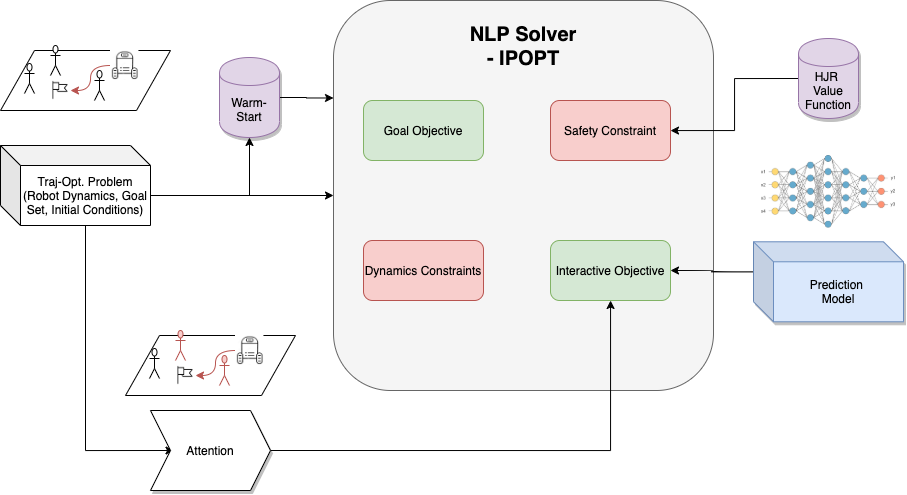
\includegraphics[width=\textwidth]{images/system.png}
\caption{System Overview}
\label{img:information_flow}
\end{center}
\end{figure}

Formally, the solution to this problem can be represented as the following optimization problem (compare Problem \ref{problem:general}), which is executed in an MPC-manner. \\

\begin{problem}{\textrm{General optimization problem}}
\begin{equation}
\min_{\u_{0:T-1}} \quad w_{goal} J_{goal} + w_{int} \sum_{k=0}^K J_{int}^k
\end{equation}
\begin{align}
\textrm{s.t. } \quad & \x_{t+1} = \f(\x_t, \u_t) & \forall t \in [0, T - 1] \\
& \xped[k] = \distmodel[k](\x_{0:t}, \xped[i]_{0:t}) & \forall k \in [0, K], \forall t \in [0, T]\\
& g_{safety}(\x_{0:T}, \xped[k]_{0:T}) \leq 0 & \forall k \in [0, K] \\
& \x_t \in \xset & \forall t \in [0, T]\\
& \u_t \in \uset & \forall t \in [0, T]\\
& \x_0 \in \xset_0
\end{align} 
\label{problem:general}
\end{problem}

Due to the linear and cheaply computable dynamics, the availability of a simulation engine tightly bound to the optimization, as the simplicity of the constraints acting on both the path $\x_{0:T}$ itself and the controls $\u_{0:T}$ are comparably "simple", as illustrated in Section \ref{text:approach/constraint}, shooting is used within this project. Therefore the trajectory is split up into several segments, one for each discrete discretization time step, which makes solving problem \ref{problem:general} more straightforward  to be solved and more robust (multiple shooting) \cite{Betts1998}. In this work the initial time $t_0 = 0$ and the final time $t_f = T \cdot \Delta t$ is used for simple notation, although not required in general \cite{Wachter2006}.
\newline
The objective function is a weighted sum of a goal-driven $J_{goal}(\cdot)$ and some interaction-driven term $J_{int}(\cdot)$, which are further explained in Section \ref{text:approach/objective}. The constraints are a combination of dynamics constraints, safety constraints as well as initial and final state restrictions, which are discussed in Section \ref{text:approach/constraint}. Note that the terminal state $\x_T$ of the planned trajectory is not constrained to be in the terminal set $\xset_f$. As stated in chapter \ref{text:introduction}, within this project, the safety and minimally impact on gait of pedestrians is considered to be more important than reaching the goal state time-optimally. While the goal-driven objective $J_{goal}(\cdot)$ introduces an incentive to approach the goal state, constraining the terminal state to be in the terminal set would informally speaking, remove the possibility of detouring to not interfere a pedestrians movement.
\newline
Over Problem \ref{problem:general} has $2*T$ optimization variables, $(2*T + 1) + 2*T + K = 3*T + K + 1$ constraints, all of them being inequality constraints, causing $T * (T+1) + 2*T + K$ non-zero Jacobian elements.

\subsubsection{Nonlinear optimization Solver} 
Since no further assumptions about the pedestrian trajectory prediction model $\distmodel[]$ have been made, the optimization is non-linear and especially non-convex in general. As shown in \cite{Gould2003}\cite{Parkinson2018}\cite{Freund2004}, there are a bunch of algorithms dealing with general non-linear optimization problems, such as line-search, trust-region, interior-point, generalized-reduced-gradient, or sequential-quadratic-programming methods as well as combinations of these such as LOQO. However, not all of them apply to constrained problems such as Problem \ref{problem:general}. For constrained optimization problems, \ac{SQP} and \ac{IPM} are the most popular ones, both having their advantages and drawbacks. While \ac{SQP} usually requires fewer solver iterations and thus fewer function calls, they scale poorly with the number of constraints and do not guarantee that intermediate results are feasible \cite{Dehdari2013}\cite{Parkinson2018}. Although this can be an advantage in computationally expensive constraints, it also leads to an infeasible solution when the algorithm is stopped before convergence. Additionally, compared to \ac{IPM}, the computational time required by the solver itself is usually larger (e.g., as demonstrated in \cite{Dehdari2013}).
\newline
In project \project, safety is induced by constraint, thus obtaining a feasible solution is crucial, also if the algorithm might be aborted before convergence due to runtime constraints. For this reason, an interior-point method has been used within the project. The idea of interior-point optimization methods is to create constraint barriers that increasingly push the solution from an infeasible state to the feasible region. IPOPT especially has shown excellent performance in smartly recovering from some infeasible state.  Therefore, it is quite robust but hard to warm-start. 
\newline
The interior-point method \ac{IPOPT}\footnote{\ac{IPOPT} is only available for C++; the cython-based wrapper cyipopt is used.} \cite{Wachter2006} has been used in many robotics applications, and has shown to be valuable even in case of very tough runtime constraints such as solving the feedforward commands in high-performance automated driving at 50 Hz in \cite{Spielberg2019} or motion planning for legged robotics \cite{Winkler2018}. Therefore it has been used in this project as well\footnote{From today's point of view, after tweaking the performance of the optimization core as best as possible, it turns out that the number of objective function calls is the bottleneck of the algorithm. Therefore comparing the capacity of the interior-point solver such as \ac{IPOPT} with \ac{SQP} solvers such as \ac{GuSTO} remains for future work.}.

% The NLP solver implements the following primal-dual methods for finding a local minimum: 1) interior-point trust-region line-search algorithm 2) active-set trust-region line-search algorithm
%Both methods can solve small-, medium-, and large-scale optimization problems efficiently and robustly. These methods use exact first and second derivatives to calculate search directions. The memory requirements of both algorithms are reduced dramatically because only non-zero elements of matrices are stored. The convergence of both algorithms is achieved by using a trust-region line-search framework that guides the iterations towards the optimal solution. If a trust-region subproblem fails to provide a proper step of improvement, a line-search is used to fine-tune the trust-region radius and ensure a sufficient decrease in objective function and constraint violations.
%The interior-point technique implements a primal-dual interior-point algorithm in which barrier functions are used to ensure that the algorithm remains feasible for the bound constraints. Interior point methods are beneficial when the optimization problem contains many inequality constraints, and you suspect that most of these constraints will be satisfied as strict inequalities at the optimal solution.
%https://documentation.sas.com/?docsetId=ormpug&docsetTarget=ormpug_nlpsolver_overview.htm&docsetVersion=14.3

\subsubsection{Implementation Details} 
The algorithm has been implemented in Python 3.7 using PyTorch \cite{pytorch}. Next to executing computations highly efficiently by vectorization and batching, PyTorch's automatic differentiation framework allows computing gradients at low computational cost as well as modular, i.e., \ without the need to define its closed-form solution explicitly. Automatic differentiation is the core of prediction-based optimization, facilitating the definition of objectives and constraints (such as $J_{int}$), which depend on a complex graph-based computation, and still being able to derive their gradient without costly and inaccurate numerical approximations.
\newline 
Furthermore, the algorithm has been implemented highly modularly, allowing to easily use pre-defined simulation environments, objective, constraint functions, or new solvers and switch between them without much knowledge about the underlying implementation. To pave the way for further research in the field, the code has been widely documented using Sphinx\footnote{Automated code documentation: https://www.sphinx-doc.org/en/master/}; for further information, please visit the \href{https://simon-schaefer.github.io/mantrap/}{project's website}.
\newline
The system's integrity has been verified by roughly 600 unit- and integration tests, secured over the code developed by the continuous integration framework CircleCI\footnote{Automated testing framework: https://circleci.com} and CodeCov\footnote{Testing coverage reports: https://codecov.io}.
